\chapter{Work performed}
\setlength{\parskip}{2.5ex plus .4ex minus .4ex}
\section{Controller}\label{sec:controller}
Each ``Controller'' associated to an agent on the world inherit from the main class ``Controller'' of SIGVerse. That is why each of them has the same dynamic shown figure~\ref{fig:controllerDyn}.\\

When the simulation starts on the SIGViewer, each ``Controller'' is initialized running ``onInit'' method. After that the ``onAction'' method is running regularly, it can be every 1 seconds like 0.1, 0.5,... It is defined by the return value of ``onAction'' method.\\
If a collision occurs between the agent and something else, ``onCollision'' is executed.\\
If the agent receives a message, ``onRecvMsg'' is executed.\\

In any case, ``onAction'' is running until the simulation stops. If the simulation restarts, ``onInit'' is not executed, the simulation continues where it stopped.\\

\noindent\begin{minipage}{\linewidth}% to keep image and caption on one page
\makebox[\linewidth]{%        to center the image
  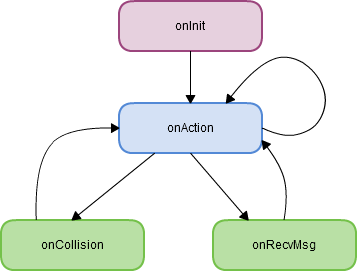
\includegraphics [width=100mm]{images/controllerDyn.png}}
\captionof{figure}{Dynamic of the ``Controller''}\label{fig:controllerDyn}%      only if needed  
\end{minipage}

\section{Architecture}
\subsection{General objective}
On the SIGServer, severals ``Controller'' can run at the same time, because there are one for each agent in the simulator and their types can be different. For exemple, we can have a ``Controller'' for a Robot and ``Controller'' for an object. The principal difference between them is that a Robot controller do not apply the same method to the agent than an object, indeed the robot can move, not an object. But they have the same dynamic, section~\ref{sec:controller}.\\
If we have three robots in the simulator, that means three ``Controller''.\\

We can see figure~\ref{fig:sig_ros_general} how the interface has to work. Several nodes can send information to topics which can be the same or not. This is the ROS part. And these topics are subscribed by the ``Controller'' of SIGServer.\\
As we can see, the same node can publish to the same node ``Topic 4'' or one node can publish to several nodes ``Node 1''.\\
However, different ``Controller'' cannot publish or subscribe to the same topic. The reason is that the ROS user do not have to write the ``Controller'' or edit it neither, it will be generated and I can not know if the user want the same behaviour between two or more agents. If the user wants this behaviour, he will have to send the same message to severals topics.\\

As we can see figure~\ref{fig:sig_ros_general} a service can be called too. The difference with publishing/subscribing is that a request is sent and the ``Controller'' will answer with a response to the node who asked ``Node 3''.

\noindent\begin{minipage}{\linewidth}% to keep image and caption on one page
\makebox[\linewidth]{%        to center the image
  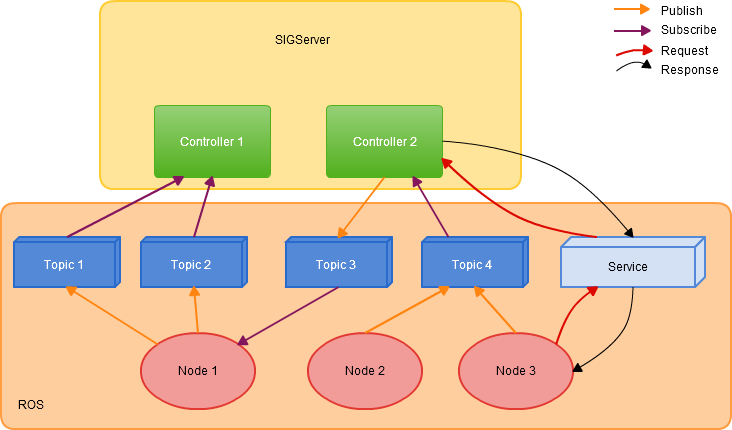
\includegraphics [width=150mm]{images/sig_ros_general.png}}
\captionof{figure}{Many ROS nodes send and receive information to many controllers}\label{fig:sig_ros_general}%      only if needed  
\end{minipage}

\subsection{Controllers used}
As explained earlier, one ``Controller'' is associated to one agent for making him act. This association is defined in the xml file which describes the agent.\\
The same ``Controller'' can be associated to several agents, that means that all agent associated to this ``Controller'' will act the same.\\
On this project, ``Controllers'' has to be developped for creating topics which sent information and make the agent acting. So, two ``Controllers'' will be necessary, one for the robot and one for the object. For generals methods like getting the all entities, they can be included on the object controller.\\
The best would be a general controller for the generals methods to avoid the duplication of topics, but for this mid-term report, only the robot controller and the object controller are implemented with the generals methods inside them.\\
So, in our case, I have as many topics (or services) for getting entities as number of agent in the simulator.\\

The robot ``Controller'' inherits from the object ``Controller'' called ``SimObjController''. The reason is that in SIGVerse, a robot is an object and has only two methods more than on the object ``Controller''.\\

\subsection{Package}
ROS is an open source framework who works with packages, every extension is a package. So, the ROS users just need to download the package wanted.\\
That is why I choose to develop a package, and only running the node called ``ros\_controller'' will be necessary to launch the SIGServer, create the ``Controllers'', the topics and services.\\
We can see figure~\ref{fig:sig_ros_package} the composition of the package.
\begin{description}
	\item[src] : The generic ``Controller'' for each kind of agent.
	\item[srv] : The definition of each services needed.
	\item[msg] : The definition of each messages needed.
	\item[tests] : Tests files to check the validity of the implementation.
\end{description}

\noindent\begin{minipage}{\linewidth}% to keep image and caption on one page
\makebox[\linewidth]{%        to center the image
  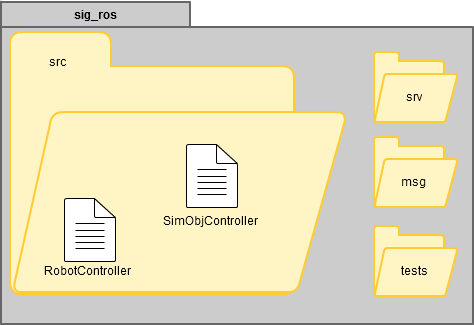
\includegraphics [width=120mm]{images/package_sig_ros.png}}
\captionof{figure}{sig\_ros package}\label{fig:sig_ros_package}%      only if needed  
\end{minipage}

\section{Usage}
From the user point of view, three steps are important, see figure~\ref{fig:usage}.\\
First, the user launches the sig\_ros package. So, the SIGServer is automatically launched and the SIGViewer can be connected.\\
Second, the user starts the simulation from the SIGViewer. So, all topics and services are created and linked to the ``Controller'' thanks to the package sig\_ros.\\
Finally, the user can create all the ROS node he wants and publish and subscribe to the topics and call services created by the step 2.

\noindent\begin{minipage}{\linewidth}% to keep image and caption on one page
\makebox[\linewidth]{%        to center the image
  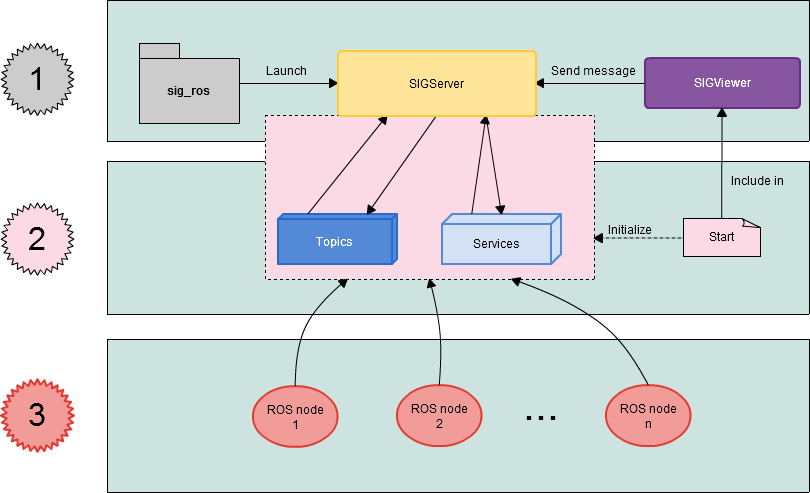
\includegraphics [width=150mm]{images/usage.png}}
\captionof{figure}{Steps to follow to start a simulation with ROS}\label{fig:usage}%      only if needed  
\end{minipage}

\section{Topics \& Services}
\subsection{Generalities}
Topics and services have to be defined. A node which subscribe to a topic receive the message as soon as it is published to the topic but no answer is given.\\
On the contrary, the service do the same as the topic bu anwser to the node who called the service.\\
The types of messages or service request can be of several simple type (double, string, ...) or a combination of these type or message created by these types.\\
It is possible to create new types, so the tranfert of SIGVerse object could be possible, but the use of the package has to be as easy as possible. So, the methods needed by the clean up task which return bad type for a message are replaced by a topic or service which execute a group of action, for exemple getPart and getPosition applied to the part are mixed in getPartPosition and the user only has to ask for a part and the position is returned with simple type ``double''.\\

The first step is to make the example of the clean up task working, so many topics and services have been created. Each of them starts by the name of the agent and follow by the name of the topic/service.

Now, we are going to see the topics and services I implemented for the robot agent, but a more exhaustive list with more details is given in annex~\ref{annex:topics} and annex~\ref{annex:services}. In those annexes, there are the topics for the robot agent but also for the object agent of the clean up task which I have started implementing.

\subsection{Topics}
The list of the topics needed for the robot agent of the clean up task is:
\begin{description}
	\item[\_onRecvMsg] : The ``Controller'' send the message received by the SIGViewer.
	\item[\_onCollisionMsg] : The name of the agent which one is in collision with are sent to this topic. If there is severals collision at the same time, severals messages are sent.
	\item[\_setWheel] : Publish the radius and the distance in a message and they will be applied to the robot.
	\item[\_setWheelVelocity] : Publish the velocity for the left and the right wheel and it will be applied.
	\item[\_setJointVelocity] : set the velocity ``angular velocity'' to the join called ``jointName''.
	\item[\_releaseObj]: Publish the part which you want to release an object and it will be done.
\end{description}

The two first topics was obvious, they are the unique topics where the ``Controller'' publish. Indeed, the dynamic of the ``Controller'' run two methods when particular events occurs, see section~\ref{sec:controller}. That is why, each time it occurs, messages are sent to this topics.


\subsection{Services}
The list of the services needed for the robot agent of the clean up task is:
\begin{description}
	\item[\_get\_time] : Get the simulation time.
	\item[\_get\_obj\_position] : Get the position of the object named name, if name is empty, return the position of the agent which the service's name start with.
	\item[\_get\_parts\_position] : Get the position of the part in parameter.
	\item[\_get\_rotation] : Get the quaternion of the agent's rotation.
	\item[\_get\_angle\_rotation] : Get the angle of the rotation of the agent.
	\item[\_get\_joint\_angle]: Get the angle between the joint.
	\item[\_grasp\_obj]: Grasp the object ``obj'' with the part ``part''.
\end{description}

\section{Internship progress}
\subsection{Discovery}
The first two weeks were dedicated to the installation of the environment: Operating System, Virtual Machine, SIGServer, SIGViewer. After that, I could see how SIGVerse works. 

Ones the environment installed, I was able to run examples of the wiki page \cite{SIGVerseWiki}. With this examples, I could see the function of the ``Controller'' and then understand how an agent can act, changing places, saying ``Hello'',... But also, how an agent communicates in both ways, sending and receiving messages.\\

After installing the environment and learning how make agents and make them move, I had to know what was ROS and how it is working. So, I installed its and I did the all beginners tutorials of the wiki page \cite{ROSWiki}.\\
After that, I could run an example of SIGVerse running with ROS and then beginning to investigate how to design an interface between SIGVerse and ROS.

\subsection{Tools \& organisation}
I'm developping on a virtual machine Ubuntu 12.04 because of the more stable version where SIGVerse works well. No IDE\footnote{Integrated Development Environment} is used, only a text editor gedit and a terminal for compilation. ROS and SIGVerse are open source so, I decided to use GitHub.\\ 
I'm using Windows 8.1 for the compatibility with the kinect which I will need by the end of the project.\\

The project was very free, my supervisor showed me the simulator SIGVerse and the first step after the installation was finding a subject. Because of the short time due to the DoW\footnote{Description of Work} deadline, I chose to work on this project.\\

Once a week, the all laboratory attends a meeting where each of members expose what he planed to do last week, what he actually did and what he will do the next week. I make my own objectives every week for achieving the main goal.\\
My supervisor answers to my questions and gives me indications during the meeting.\\

I make unit tests with ROS to be sure of the good functioning.

\subsection{Schedule}
\subsubsection{What I planned}
In the DoW report, I planned to achieve the job L2 before the mid-term report deadline. That means make SIGVerse works with ROS by a simple way like one ``Controller'' with one node and generate a ``Controller'' for each agent on the simulator.\\

For the next months, I planned to design and develop the topics and services that are necessary to control the agents. I also planned to make an interface between the real human and the simulator. For example, making work the kinect. We can see figure~\ref{GanttChart} the schedule of the DoW.
\subsubsection{What I did}
Finally, this part was easier than I though and I could start the next job. So, I started implementing some topics and services for the clean up task.\\
Only the methods for the clean up task have been done and some others. You can see at \url{https://www.youtube.com/watch?v=PL4MCjire2M&feature=youtu.be} a demonstration of the clean up task. The all actions of the robot are sent by ROS.\\

For the next months, I will follow the DoW schedule, starting with finishing the clean up task example. The time saved by the first two month will be usefull for making more tests.

\subsubsection{Troubles}
During this two first month, I had to solve some troubles.\\
First of all, due to my lack of knowledge about ROS, it was very difficult to gain a full view of the project at the beginning. That is why, I had to spend some days to learn from the ROS tutorials and to practice with this framework.\\
When I started implementing the ``Controller'', I had a problem of inheritance. Indeed, I had to inherit the robot ``Controller'' from the object ``Controller'' and keep this two ``Controller'' usable for an agent. This inheritance was not easy because of ROS.\\
I found a SIGVerse bug using a function ``getSimulationTime()''. I spent a lot of time diagnosing this bug because I though it came from my code but finally it was a SIGVerse error. So, I made a bug report.\\
The documentation of SIGVerse is in japanese, so it is quiet difficult to understand what every method does, so I did a lot of tests to figure it out.
%Trois importantes réunions ont eu lieu. Une en début de stage le 27 juin avec l'équipe VLE qui avait pour but de définir la manière d'intégrer les nouvelles fonctionnalités au logiciel GVLE.\\
%Une seconde a eu lieu le 9 août par l'intermédiaire de jipsi\footnote{Système de visioconférence} avec les principaux futurs utilisateurs, du plugin IBM afin de faire un état d'avancement.\\
%Pour la dernière réunion, le 4 août, ces principaux utilisateurs sont venus sur le site de Toulouse afin que je leur explique le fonctionnement du plugin.
%
%\vspace{-10cm}
%\begin{landscape}
%%\thispagestyle{empty}
%%\thispagestyle{plain}
%\setlength{\topmargin}{25pt}
%\titlespacing{\subsection}{0cm}{0cm}{0cm}
%
%
%\noindent\begin{ganttchart}[
%hgrid,
%vgrid,
%inline,
%time slot format=stardate
%]{2014.167}{2014.215}
%\gantttitlecalendar{year, month=name, day} \\
%\ganttbar{Compréhension du sujet}{2014.167}{2014.188}
%\ganttbar{Developpement fenêtre principale du plugin}{2014.189}{2014.206}
%\ganttbar{Mise en place proxy lua}{2014.207}{2014.215}\\
%\ganttbar{Lecture documentation}{2014.167}{2014.174}
%\ganttmilestone{Réunion d'organisation}{2014.177}
%\ganttbar{Prise de connaissance du code source}{2014.180}{2014.200}\\
%\ganttbar{Réalisation du TP Forrester}{2014.170}{2014.185}
%\ganttbar{Debogage}{2014.202}{2014.215}
%\end{ganttchart}
%
%\noindent\begin{ganttchart}[
%hgrid,
%vgrid,
%inline,
%time slot format=stardate
%]{2014.216}{2014.264}
%\gantttitlecalendar{year, month=name, day} \\
%\ganttbar{Développement extensions lua}{2014.216}{2014.230}
%\ganttbar{Rapport de Stage}{2014.230}{2014.252}
%\ganttbar{Congé}{2014.253}{2014.263}\\
%\ganttmilestone{Réunion d'avancement}{2014.220}
%\ganttbar{Mise en place du Scheduler}{2014.223}{2014.231}
%\ganttbar{Modification GUI}{2014.233}{2014.238}
%\ganttmilestone{Présentation du plugin}{2014.246}\\
%\ganttbar{Tests}{2014.218}{2014.244}\\
%\ganttbar{Debogage}{2014.216}{2014.250}
%\end{ganttchart}
%\end{landscape}

